
\chapter{First principle methods}




\section{The twin test}


Suppose we are given samples $\mathcal{D} = \{x_i, y_i\}_{i \in [n]}$ from an ANM $X \rightarrow Y$, which recall has the form

\[
    \begin{cases} 
        & Y = f(X) + Z \\
        & X \bigCI Z,\quad X \thicksim p_X,\quad Z \thicksim p_{Z}  
     \end{cases}  
\]

The main strategy of most causal inference methods has been to estimate $f$, and then to compute the estimated
residual $\hat{e} = \hat{f}(x) - y$; the final step is to test the independence between $\hat{e}$ and $X$. This exploits 
the assumption that $X \bigCI Z$. In practice we often have that the noise is \textit{independent}, 
i.e. we produce a sequence $Y_1, ..., Y_n$, where $Z_i \bigCI Z_j$ $\forall i \neq j$.

By directly exploiting the IID noise assumption, we will circumvent the need for an independence test. The 
idea is to to partition the data -- for simplicty you can think about splitting it around the median; we 
then estimate the residuals for each partition, and we then test if the IID noise assumption holds by comparing
the residuals of each partition. We can apply this procedure to both directions and then we will call the 
direction causal if it's residuals are more similar. 

We will explain this idea in more detail by following an example: we are given samples 
$\mathcal{D} = \{x_i, y_i\}_{i \in [n]}$ from an ANM $X \rightarrow Y$; 
We first visualise the data $\{x_i, y_i\}_{i \in [n]}$, by plotting
X to Y, and viceversa (see Figure \ref{fig:algo_data}). 

\begin{figure}[H]
    \captionsetup[subfigure]{labelformat=empty}
    \centering
    \subfloat{{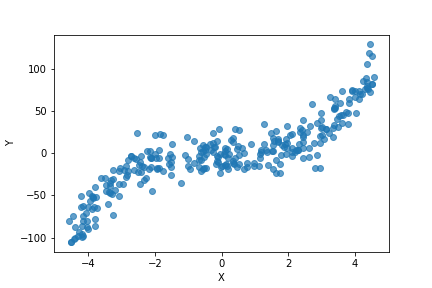
\includegraphics[width=6.5cm]{algo_direct.png} }}%
    % \quad
    \subfloat{{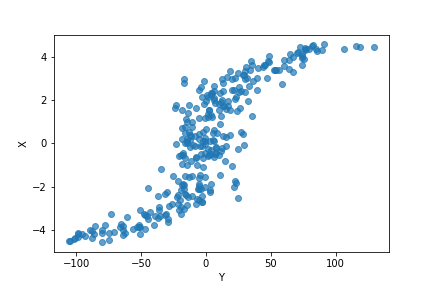
\includegraphics[width=6.5cm]{algo_reverse.png} }}%

    \caption{300 samples of data $X$, $Y$. With \textbf{ANM}: \\
    $f(x) = \tanh(x) + 2\sin(2x) + x^3$}
    $X \thicksim \mathcal{U}_{[-a, a]}$ and $Z \thicksim \mathcal{N}(0, \sigma^2)$
    \label{fig:algo_data}
\end{figure}



For simplicty assume $X \thicksim \mathcal{U}_{[-a, a]}$ (i.e. $X$ is uniformly disributed), then we can split 
the data in two, say $D_1$ and $D_2$, where we place all samples with $x_i < 0$ into $D_1$, and the rest into 
$D_2$. To be more precise, $\mathcal{D}_1 = \{(x_i, y_i) : x_i < 0\}$ and $\mathcal{D}_2 = \mathcal{D} 
\backslash \mathcal{D}_1$. We also do the same procedure for the reverse set up, i.e. we reverse the roles of x and y
, $\mathcal{\tilde{D}} = \{y_i, x_i\}_{i \in [n]}$ and by the same procedure we obtain $\mathcal{\tilde{D}}_1$
and $\mathcal{\tilde{D}}_2$. We can visualise this parition bellow in Figure \ref{fig:colo_code}.
 
\begin{figure}[H]
    \captionsetup[subfigure]{labelformat=empty}
    \centering
    \subfloat[Partitions $D_1$ and $D_2$]{{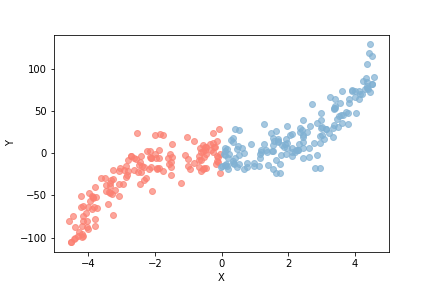
\includegraphics[width=6.5cm]{algo_part.png} }}%
    % \quad
    \subfloat[Partitions $\mathcal{\tilde{D}}_1$ and $\mathcal{\tilde{D}}_2$]{{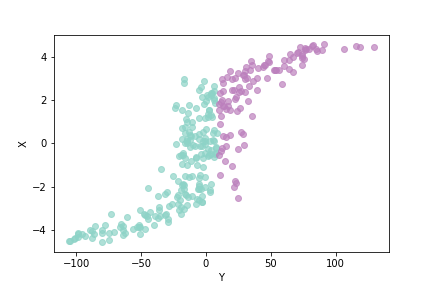
\includegraphics[width=6.5cm]{algo_part_reverse.png} }}%
    \caption{ We highlight each partition in a different color. On the left we have $D_1$ and $D_2$; and on 
    the right we have $\mathcal{\tilde{D}}_1$ and $\mathcal{\tilde{D}}_2$ }
    \label{fig:colo_code}
\end{figure}

If we estimate a fit $\hat{f}_1$ for $\mathcal{D}_1$ and similarly $\hat{f}_2$ for $\mathcal{D}_2$, then we can 
compute residuals for each sets, say $\hat{e}_1$ for $\mathcal{D}_1$  and $\hat{e}_2$ for $\mathcal{D}_2$.
Since the noise is -- not only independent from $X$ but also -- iid, it follows that $\hat{e}_1$ and $\hat{e}_2$
follow the same distribution -- assuming a perfect fit $f$. We can viualize this by looking at the 
histograms from the residuals.

\begin{figure}[H]
    \captionsetup[subfigure]{labelformat=empty}
    \centering
    \subfloat{{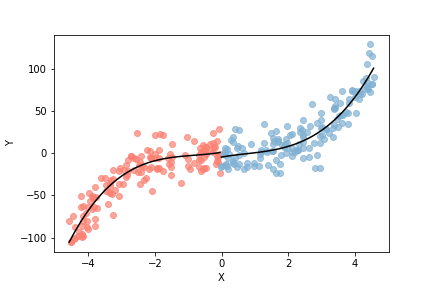
\includegraphics[width=6.5cm]{algo_fit_direct.png} }}%
    % \quad
    \subfloat{{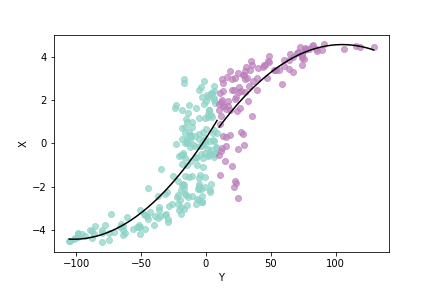
\includegraphics[width=6.5cm]{algo_fit_reverse.png} }}%
    % \caption{Samples from two different sources, $X$ and $Y$, how can we tell if 
    % they come from the same distribution?}
    \\

    \subfloat{{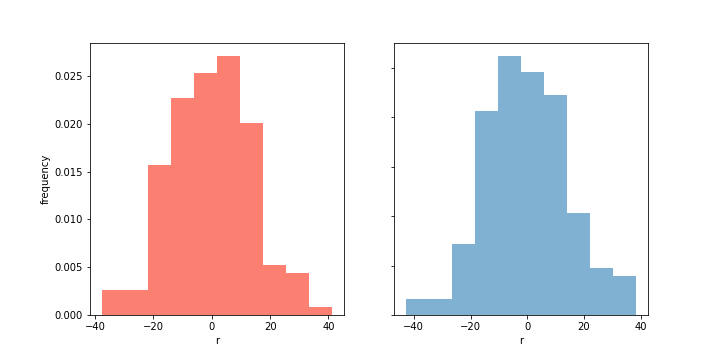
\includegraphics[width=6.5cm]{algo_res_direct.png} }}%
    % \quad
    \subfloat{{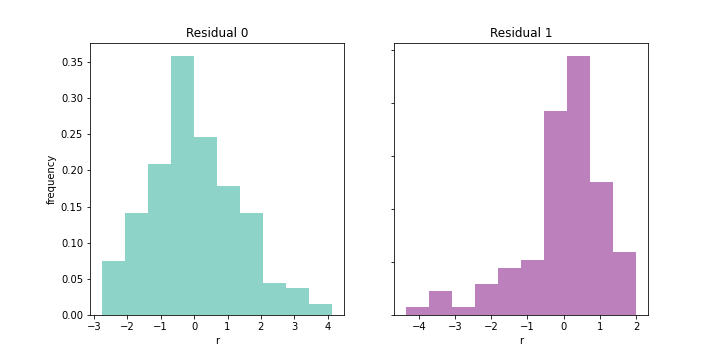
\includegraphics[width=6.5cm]{algo_res_reverse.png} }}%

    \caption{  We show the the estimated fits $\hat{f}$ for each parition in black. Bellow each 
    partition we plot the histograms of the residuals -- in the same color. }
    \label{fig:algo_fit}
\end{figure}

Note that for the reverse model, the noise in $\mathcal{\tilde{D}}_1$ appears to be very different from 
that of $\mathcal{\tilde{D}}_2$; this is not a coincidence -- intuitvely, it seems very unlikely that 
regressing in the other direction will also result in independence noise. Further, as we briefly 
mentioned in the early chapters, as \cite{hoyer2009nonlinear} show, it is unlikely that for a non-linear 
we might not have identifiability. 

One simple idea is then to quantify these observations; from $\mathcal{D}_1$ and $\mathcal{D}_2$ we 
compute $\hat{e}_1$, $\hat{e}_1$, and so we can define as a score for these sets:

$$
     \mathcal{C}(\mathcal{D}_1, \mathcal{D}_2) = \norm{p_1 - p_2}_1
$$

Where $p_1$ is the empirical distribution of $\hat{e}_1$, and similarly for $p_2$ and $\hat{e}_2$. We 
can then apply the score function to $\mathcal{\tilde{D}}_1$ and $\mathcal{\tilde{D}}_2$ and 
infer causality as follows:

\[ 
     \begin{cases} 
        & X \rightarrow Y \quad  \mathcal{C}(\mathcal{D}_1, \mathcal{D}_2) 
        \leq \mathcal{C}(\mathcal{\tilde{D}}_1, \mathcal{\tilde{D}}_2) \\
        & Y \rightarrow X \quad \text{otherwise}
     \end{cases}
\]

In the above example, we get that $\mathcal{C}(\mathcal{D}_1, \mathcal{D}_2) = 0.138$ and that
$\mathcal{C}(\mathcal{\tilde{D}}_1, \mathcal{\tilde{D}}_2) = 0.480$ where use bins of size $5$ 
for discretization; We are able to predict the causal direction with high confidence.

Assuming the regressions are \textbf{faithfull}, then as $n \rightarrow \infty$ we know that both 
$p_1$ and $p_2$ will converge to the same $p_Z$ and so $\mathcal{C}(\mathcal{D}_1, \mathcal{D}_2) \rightarrow 0$.
On the other hand, it is unlikely that the residuals of $\mathcal{\tilde{D}}_1$ and $\mathcal{\tilde{D}}_2$ 
follow the same distribution (due to the non-linearlities introduced by f and the additivy of the noise) and 
so we can be pretty confident that asympotically the procedure will correct. In fact, assuming that \textbf{ANM}
$X \rightarrow Y$ is identifiabile will be enough to show that this procedure is consistent.

In essence the algorithm consists of the parts:

\begin{enumerate}
    \item Partition the data
    \item Estimate regressions and residuals
    \item Compute scores
\end{enumerate}

Before giving the general description of the algorithm we will comment on each of these parts in more detail. 

\subsection{Partition}

Say that we partition $\mathcal{D}$ into $\mathcal{D}_1, ..., \mathcal{D}_k$; then these 
partitions need to satisfie three requirements:

\begin{enumerate}
    \item The partitions need to be \textbf{dense}: 
    $|\mathcal{D}_i| \geq \rho |\mathcal{D}|, \quad \forall i \in [k]$, for some $\rho \in (0, 1)$.
    \item The partitions need to be disjoint 
    $$
    \mathcal{D} = \bigcup_i \mathcal{D}_i \quad \text{and} \quad
    \mathcal{D}_i \cap \mathcal{D}_j = \emptyset \quad \forall i \neq j
    $$
    \item We need to be able to order the paritions, say $\mathcal{D}_1, ..., \mathcal{D}_k$, such that
    if $i < j$ then\footnote{The $*$ is to indicate a dummy variable, as we do not care for the value of $y$.}: 
    $$
    \operatorname{max} \{ x : (x, *) \in \mathcal{D}_i \} \leq 
    \operatorname{min} \{ x : (x, *) \in \mathcal{D}_j \}
    $$
\end{enumerate}

The first condition -- that of dense partitions -- is to avoid getting trivial large deviations between residuals 
in the subsets; the second reason is that if they are dense, then we can give asymptotic guarantees about each subset.
The second and third conditions simply ensure that we are not mixing data and that it is coherent to make regression
in each subset. 

If we use K-means (perhaps the most popular clustering algorithm), then conditions 2. and 3. are met. The only 
questions is in regards to conditions 1. K-means starts by randomly initialisting two or n centers (depending 
on the number of clusters that we want), and the updates the centers that they locally 
minimizes within-cluster variances. If our data is infinite support, and we re-run K-means if there is some cluster
$i$ s.t. $|\mathcal{D}_i| < \rho |\mathcal{D}|$; then if we have enough data and for some $\rho$ we can be quite 
certain that the algorithm will eventually terminate. 

In practice this has always been the case (for $\rho = .3$); so we conjecture that one can prove the above statement 
rigorously. 

The last question is, "How many clusters do we want?". Obviously for the small data regime we must be content 
wuth only two clusers; but what if we have a lot of data? As we will see, we observe experimentally that if we 
we choose the number of partition as an increasing function w.r.t. sample size, then we can get better accuracies.

One reason that more partitions are desirable is that then the regression problem becomes easier; Indeed, as we 
zoom into a function it tends to become smoother.


\subsection{Regression}

A benefit of partitioning the is that we are also partitioning the function we are trying to estimate; in 
particular one would expect that the regression will be easier, e.g. a low order polynomial might be enough.

We do elementary model selection, we take the best model with BIC score for degrees 1 to 6. 

Show example of many partitions

\subsection{Score functions}

We have seen in previous chapters various ways to measure the distances between two distribtions say 
$p_1$ and $p_2$, via some score function $\mathcal{D}(p_1, p_2)$; for example $\mathcal{D}$ could be the 
MMD metric, or the $l_1$ distance.

Now instead we have a set of distributions, say $P_k = p_1, ..., p_k$, and we wish to see how homogenous
$P_k$ is compared to some other set $\tilde{P}_j$ -- recall that we wish to see in which of the two, 
 the distribtions are more likely to be the same, i.e. we are testing the iid assumption. 

There are several simple ways to go about this:

$$
    C(P_k) = \operatorname{max}_{i, j} \mathcal{D}(p_i, p_j)
$$

Another option is to take an average of the pairwise score:

$$
    C(P_k) = \frac{1}{\binom{k}{2}} \sum_{i < j} \mathcal{D}(p_i, p_j)
$$

or even 

$$
    C(P_k) = \frac{1}{\binom{k}{2}} \sum_{i < j} \mathcal{D}(p_i, p_\mu)
    , \quad p_\mu = \frac{1}{k} \sum_i p_i
$$


Thus if $C(P_k) < C(\tilde{P}_j)$, we can say that the distributions in $P_k$ are
more homogenous; e.g. they more likely to produce similar looking noise. 

We have tested all of the above and find that the first method -- using the maximum score between pairs --
gives the best performance.

\subsection{Algorithm}

We note that the algorithm is a general framework as we are free to choose the partition, regression method
and score function. We would like to point out that we recycle the data, i.e. we use the same data for 
estimating the regression and subsequent score function; obviously if one wishes one can easily split the 
data in the paritions to use a different portion of the data for estimation and for evaluating the score function.

\begin{algorithm}[H]

    \caption{\textbf{Twin method}: General procedure to decide whether $p_{x, y}$ satisfies and ANM $X \rightarrow Y$
        or $Y \rightarrow X$}
  
    \textbf{Input}:

    \begin{enumerate}
        \item I.i.d samples $\mathcal{D} = \{ (x_i, y_i )\}_{i \in [N]}$ of $X$ and $Y$
        \item Partition procedure
        \item Regression method
        \item Score estimator $\hat{C}: R^{* \times *} \rightarrow \R$, where E is a set of vectors. 
    \end{enumerate}
    
    \textbf{Output}: $\hat{C}_{X \rightarrow Y}$, $\hat{C}_{Y \rightarrow X}$, dir

    \begin{enumerate}

        \item $\tilde{\mathcal{D}} := \{ ( y_i, x_i )\}_{i \in [N]}$

        \item \textbf{Partition} the data into subsets\footnote{The subsets are disjoint and their union equals the data}:
        \begin{itemize}
            \item[--] $\{ \mathcal{D}_i \}_{i \in [k]} \quad \text{s.t.} \quad \mathcal{D}_i \subset \mathcal{D}, 
            \forall i \in [k]$
            \item[--] $\{ \tilde{\mathcal{D}}_i \}_{i \in [j]} \quad \text{s.t.} \quad \tilde{\mathcal{D}}_i 
            \subset \tilde{\mathcal{D}}, \forall i \in [j]$
            \item[--] Where integers $j, k > 1$ are determined by the partition procedure.
        \end{itemize}

        \item \textbf{Estimate regressions} and residuals for each subset
        
        for $i \in [k]:$

        \begin{itemize}
            \item[--] Let $\mathbf{x}$, $\mathbf{y}$ be the vectors formed from $\mathcal{D}_i$
            \item[--] $\hat{f}_Y$ of the regression function $x \mapsto \E(Y | X=x)$
            \item[--] $ \mathbf{\hat{e}_{Y}}(i) := \mathbf{y} - \hat{f}_Y(\mathbf{x})$
        \end{itemize}

        end for

        $\mathbf{E_Y} := \{ \mathbf{\hat{e}_{Y}}(i) \}_{i \in [k]} $

        for $i \in [j]:$

        \begin{itemize}
            \item[--] Let $\mathbf{x}$, $\mathbf{y}$ be the vectors formed from $\tilde{\mathcal{D}}_i$
            \item[--] $\hat{f}_X$ of the regression function $x \mapsto \E(X | Y=y)$
            \item[--] $ \mathbf{\hat{e}_{X}}(i) := \mathbf{x} - \hat{f}_X(\mathbf{y})$
        \end{itemize}

        end for

        $\mathbf{E_X} := \{ \mathbf{\hat{e}_{X}}(i) \}_{i \in [j]} $

        \item \textbf{Compute scores} to measure the difference between the residuals
        \begin{itemize}
            \item[--] $\hat{C}_{X \rightarrow Y}: = \hat{C}( \mathbf{E_Y} )$ 
            \item[--] $\hat{C}_{Y \rightarrow X}: = \hat{C}( \mathbf{E_X} )$
        \end{itemize}        

        \item Output $\hat{C}_{X \rightarrow Y}$, $\hat{C}_{Y \rightarrow X}$, and
        
        \[ 
        \text{dir} :=  
         \begin{cases} 
            & X \rightarrow Y \quad \text{if} \; \hat{C}_{X \rightarrow Y} \leq \hat{C}_{Y \rightarrow X}\\
            & Y \rightarrow X \quad \text{otherwise}
         \end{cases}
        \]
        
    \end{enumerate}

  \label{alg:twin_test}
  \end{algorithm}


\subsection{Consistency}

We will show consistency for a simple set up of the twin test -- but we note that generalising it to the more 
general set up should be direct from our proof. 


The setup was the linear \textbf{ANM}:

\[ \begin{cases} 
    & Y = f(X) + Z  \\
    & X \bigCI Z,\; X \thicksim p_x,\; Z \thicksim p_{Z}  
 \end{cases}
\]

In practice we are given samples $\mathcal{D} = \{x_i, y_i\}_{i \in [n]}$ from an ANM $X \rightarrow Y$; next 
the algorithm will proceed to split the data into sets $\mathcal{D}_1$ and $\mathcal{D}_2$. It then proceeds 
to compute residuals and compute some scores between them.

To simplify the proof, we will \textbf{skipe the partition procedure} and assume that
we are directly given $\mathcal{D}_1$ and $\mathcal{D}_2$, each with 
$n$ samples (Note that, if $p_x$ is uniform, then having these sets be of equal size would happen exponentially 
fast; indeed, in general, we will have dense partitions). 

Next, we will assume that on each interval, the data is linear with slope $a_1$ and $a_2$ resp. 

\begin{figure}[!h]
    \centering
    \begin{tikzpicture}
        \draw[thin, dashed] (1.5, -0.5) -- (1.5, 2.6) node[above] {};
        \path (0.75, -0.8) -- (0.75, -0.6) node[above] {$\mathcal{D}_1$};
        \path (2.25, -0.8) -- (2.25, -0.6) node[above] {$\mathcal{D}_2$};
        \draw[->] (-1, 0) -- (4.2, 0) node[right] {$x$};
        \draw[->] (0, -1) -- (0, 3) node[above] {$y$};
        \draw[scale=1, domain=0:1.5, smooth, variable=\x, blue] plot ({\x}, {0.5*\x});
        \draw[scale=1, domain=1.5:3, smooth, variable=\y, red]  plot ({\y}, {1*\y - 0.75});
        \draw[decoration={brace,mirror,raise=5pt},decorate] (0.1, -.5) -- node[below=8pt] {$\mathcal{D}$} (2.9, -.5) ;
      \end{tikzpicture}
      \caption{Slopes $a_1$ and $a_2$ in blue and red respectively.}
\end{figure}

Thus our problem can be seen as getting data from two difference \textbf{ANM}, both with identical noise, but with 
a different truncation of $X$:

$\mathcal{D}_1$ is sampled from 

\[ \begin{cases} 
    & Y_1 = a_1 X_1 + Z  \\
    & X_1 \bigCI Z,\; X_1 \thicksim p_{X_1},\; Z \thicksim p_{Z}  
 \end{cases}
\]

and $\mathcal{D}_2$ is sampled from 

\[ \begin{cases} 
    & Y_2 = a_2 X_2 + Z  \\
    & X_2 \bigCI Z,\; X_2 \thicksim p_{X_2},\; Z \thicksim p_{Z}  
 \end{cases}
\]

Note that without loss of generality we can assume $X_1 \thicksim X_2 \thicksim X \thicksim P_X$.

We will call this scenario the \textbf{simplified Twin Test scenario}. 

We next describe the steps of the algorithm after partitioning:

We first split $\mathcal{D}_1$ in two sets of equal size $\mathcal{D}_{1}^{train}$ and 
$\mathcal{D}_{1}^{test}$. We first use $\mathcal{D}_{1}^{train}$ to estimate $a_1$, say $\hat{a}_1$ via 
regression. Then, using $\mathcal{D}_{1}^{test}$, we estimate the residual:

$$
    \hat{Z}_1 = Y_1 - \hat{a}_1 X
$$

We then discretise $\hat{Z}_1$ and form a distribution say $\hat{p}_1$; we can do the same thing for 
$\mathcal{D}_2$, and by doing the same procedure obtain $\hat{p}_2$.

We discretise both with a fixed step size, say $s$; as we will see, the only requirement is that we fix 
the size beforehand.

We use the $l_1$ distance as our score:

$$
    \hat{C}_{X \rightarrow Y} = \norm{\hat{p}_1 - \hat{p}_2}_1
$$

As we have seen, $\hat{C}_{Y \rightarrow X} > 0$ holds in general except in very particular situations. So, 
to prove that our algorithm is consistent, we need to show that:

$$
    \hat{C}_{X \rightarrow Y} \rightarrow 0 \qquad \text{as }  \qquad n \rightarrow \infty
$$

This is precisely what we will show:

\begin{theorem}
    The \textbf{simplified Twin Test scenario}t is consistent, i.e. 

$$
    \hat{C}_{X \rightarrow Y} \rightarrow 0 \qquad \text{as }  \qquad n \rightarrow \infty
$$
\end{theorem}

The idea of the proof is to observe the following:

If we have enough data, i.e. when $n$ is large enough then assuming the regression is 
faithfull, we can chose any $\alpha$ such that

$$
    \abs{a_1 - \hat{a}_1} \leq \alpha \qquad \text{and} \qquad \abs{a_2 - \hat{a}_2} \leq \alpha
$$

This means that 

$$
    \hat{Z}_1 = Z + (a_1 - \hat{a}_1)X \quad \implies \quad Z - \alpha X \leq \hat{Z}_1 \leq Z + \alpha X 
$$

and similarly

$$
    \hat{Z}_2 = Z + (a_2 - \hat{a}_2)X \quad \implies \quad Z - \alpha X \leq \hat{Z}_2 \leq Z + \alpha X 
$$

Note that $\hat{Z}_1 \thicksim P_{Z + \Delta_1 X}$ and $\hat{Z}_2 \thicksim P_{Z + \Delta_2 X}$ , where for 
brevity we denote $\Delta_1 = a_1 - \hat{a}_1$ and $\Delta_2 = a_2 - \hat{a}_2$. We can visualise the distance
between these distribtions as follows: (see\footnote{Note that the illustration does not follow the actual
gemoetry of the space, we draw it solely to gain intuition about the problem.} figure \ref{fig:dist})

\begin{figure}[!h]
    \centering
    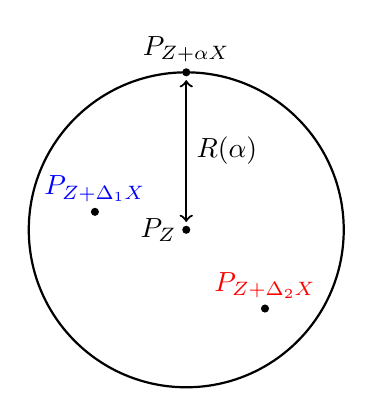
\begin{tikzpicture}[scale=2]
        \draw[thick] (0,0) circle (1);
        \draw[semithick, fill=black] (0,0) circle (0.02) node[left] {$P_Z$};
        \draw[thick, <->] (0, .05) -- node[right] {$R(\alpha)$} (0, .95);
        \draw[semithick, fill=black] (0,1) circle (0.02) node[above] {$P_{Z + \alpha X}$};
        % p_1 and p_2
        \draw[semithick, fill=black] (.5, -.5) circle (0.02) node[above, color=red] {$P_{Z + \Delta_2 X}$};;
        \draw[semithick, fill=black] (-.58, .114) circle (0.02) node[above, color=blue] {$P_{Z + \Delta_1 X}$};;
      \end{tikzpicture}
      \caption{The $l_1$ "ball" around $P_Z$, for brevity we denote 
      $\Delta_1 = a_1 - \hat{a}_1$ and $\Delta_2 = a_2 - \hat{a}_2$}
      \label{fig:dist}
\end{figure}

The idea is then the following, given some $\epsilon > 0$, we want to show that asympotically

$$
    \norm{\hat{p}_1 - \hat{p}_2}_1 > \epsilon
$$

cannot happen. The game plan will be to find a bound on the $R(\alpha)$; once we have one, we are done, we 
will simply pick an $\alpha$ s.t. $R(\alpha) < \epsilon$. Recall that $\alpha$ is the error in of our $\hat{a}$
estimate, which we can get arbitrarily small with enough samples. 

We begin by proving lemmas to find bounds for the radius $R(\alpha)$.

\begin{lemma} Given $\alpha, \delta > 0$, random variables $Z$ and $X$ s.t. $\alpha X + Z$, where $X \bigCI Z$, 
$X \thicksim P_X$, $Z \thicksim P_Z$, with $\int P_{Z}^{\prime}(t) d t < \infty$.
$\alpha X + Z \thicksim  P_{\alpha X + Z}$, there is some $C > 0$ s.t.

$$
\left\|P_{Z} -  P_{\alpha X + Z} \right\|_{1} \leqslant \alpha C + \delta
$$
\label{lemma:conv_bound}
\end{lemma}

\begin{proof}
    ~

First note that $\alpha X \thicksim \frac{1}{\alpha}P_{X} \left( \frac{\tau}{\alpha} \right)$ by applying the 
change of variable rule. 

Next, since $X \bigCI Z$, we may write $P_{\alpha X + Z}$ as a convolution:

$$
    P_{\alpha X + Z} (t) = \int P_{Z}(t-x) \frac{1}{\alpha}P_{X} \left( \frac{x}{\alpha} \right) d x =
     \int P_{Z}(t-\alpha x) P_{X}(x) d x
$$

Let $T^{\alpha X} P_Z(t) := P_{Z}(t-\alpha x)$ (we use the notation introduced by Lagrange for the shift operator).

Hence we may write (with $P_X$ as the underlying measure):

$$
    P_{\alpha X + Z} (t) = \E\left[P_{Z}(t-\alpha X ) \right]
$$


We proceed as follows:

$$
\begin{aligned}
\norm{P_{Z}- P_{\alpha X + Z}}_{1} &=\int\abs{ P_{Z}(t)-\E\left[P_{Z}(t-\alpha X ) \right]} d t \\
&\leq \int \E \abs{ P_{Z}(t)-P_{Z}(t-\alpha X )} d t \\
&=\E \int\abs{ P_{Z}(t)-P_{Z}(t-\alpha X ) } d t \\
&= \E \left[ \norm{P_{Z}- T^{\alpha X} P_Z }_{1} \, | \, \abs{X} \leq k \right] 
P\left( \abs{X} \leq k \right) + \E \left[ \norm{P_{Z}- T^{\alpha X} P_Z }_{1} \, | \, \abs{X} > k \right] 
P\left( \abs{X} > k \right) \\
&\leq \E \left[ \norm{P_{Z}- T^{\alpha X} P_Z }_{1} \, | \, \abs{X} \leq k \right] 
 + 2 P(\abs{ X} > k) \\ 
&\leq \int\abs{ P_{Z}(t)-P_{Z}(t-\alpha C^* ) } d t + 2 P(\abs{ X} > k) \\
&\leq \int\abs{ P_{Z}(t)- (P_{Z}(t) + \alpha C^* P_{Z}^{\prime}(t)) } d t  + 2 P(\abs{ X} > k)\\
&\leq \alpha C^* \int P_{Z}^{\prime}(t) d t + 2 P(\abs{ X} > k)\\
&\leq \alpha C + \delta
\end{aligned}
$$

The first equality follows by the aforementioned observation. The first inequality follows from the triangle 
inequality; 
the equality that comes after is due to Fubini's theorem, we can swap the expectation (which is also an 
integration) since all measures are measurable. We next use the law of total probability by splitting 
the expectation w.r.t some $k$ to be chosen later.  

The next upper bounds follows by noting that
$\norm{p - q}_1 \leq 2$ for any distribtions $p$ and $q$. Next observe that 
$\E \left[ \norm{P_{Z}- T^{\alpha X} P_Z }_{1} \, | \, \abs{X} \leq k \right]$ is the average $l_1$ distance
between $\norm{P_{Z}}$ and random shifts of itself. Hence if we choose the shift as follows:

$$
    C^* = \operatorname{argmax}_{s \in [-k, k]} = \int\abs{ P_{Z}(t)-P_{Z}(t-\alpha s ) } d t 
$$

we can upper bound the average distance by the largest $l_1$ distance between any shift; 
note that there is at least one maximiser since we are optimising over a compact set. 

TODO -- Taylor approx bound -- 

We next approximate $P_{Z}(t-\alpha C^* )$ by using it's taylor expansions -- this is justified by the fact 
that we will pick $\alpha \approx 0$.

Using taylor expansions we get that:

$$
    P_{Z}(t-\alpha C^* ) = P_{Z}(t) + \sum_{n \geq 1} \left( \alpha C^* \right)^n P_{Z}(t)^{(n)}
$$

Note that in our original equation this means that we need to bound


$$
     \sum_{n \geq 1} \left( \alpha C^* \right)^n \int P_{Z}(t)^{(n)} dt
$$

Note that we can pick any $\alpha$, indeed we will later make it smaller than $\epsilon$. But I am 
not sure how to bound the derivatives of the pdf...

TODO -- Taylor approx bound end -- 

Finally, since we can pick $k$, we choose it large enough s.t. $2P(\abs{ X} > k) \leq \delta$, we then let 
$C = C^* \int P_{Z}^{\prime}(t) d t$ and we are done.

We note that while $C^*$ will depend on $\delta$, this is not a problem. We will first pick $\delta$ to be 
some small constant, this will then determine $C^*$ to be some other constant; after this we will be choose 
$\alpha$. 
\end{proof}

The next lemma will also be important 

\begin{lemma}
    Let $P$ and $Q$ be two distribtions, then let $P^*$, $Q^*$ resp. be discretized versions. Then if 
    $\norm{P - Q}_1 \leq \delta$ for some $\delta$, then

    $$
        \norm{P^* - Q^*}_1 \leq \delta
    $$
    \label{lemma:quantisation}
\end{lemma}

\begin{proof}
    ~
    Using the data processing inequality (lemma \ref{lemma:dpi}), and noting that one can express the $l_1$
    distance as a divergence proves the claim. 
\end{proof}

We can now conclude by proving consistency

\begin{proof}

\begin{align*}
        P\left( \norm{ \hat{p}_1 - \hat{p}_2 }_1 \geq \epsilon \right) &\leq 
        P\left( \norm{ \hat{p}_1 - p_Z}_1 + \norm{ \hat{p}_2 - p_n}_1 \geq \epsilon \right) \\
        &\leq P\left( \norm{ \hat{p}_1 - p_Z}_1 + \norm{ \hat{p}_2 - p_Z}_1 \geq \epsilon 
        \; | \; \abs{a_1 - \hat{a}_1} \leq \alpha \; \text{,} \; \abs{a_2 - \hat{a}_2} \leq \alpha \right) \\
                        &\qquad + P\left( \abs{a_1 - \hat{a}_1} > \alpha \; \text{or} \; \abs{a_2 - \hat{a}_2} > \alpha  \right) 
\end{align*}

The first inequality follows by the triangle inequality, and the second one by using the law of total probability.

Observe that 

$$
P\left( \abs{a_1 - \hat{a}_1} > \alpha \; \text{or} \; \abs{a_2 - \hat{a}_2} > \alpha  \right)  =
P\left( \abs{a_1 - \hat{a}_1} > \alpha \right) + P \left( \abs{a_2 - \hat{a}_2} > \alpha  \right) 
$$

Both of which go to zero assuming that we have a suitable regression. 

It remains to bound 

\begin{equation}
    P\left( \norm{ \hat{p}_1 - p_Z}_1 + \norm{ \hat{p}_2 - p_Z}_1 \geq \epsilon 
        \; | \; \abs{a_1 - \hat{a}_1} \leq \alpha \; \text{,} \; \abs{a_2 - \hat{a}_2} \leq \alpha \right)
\end{equation}

Note that $\hat{p}_1 \rightarrow P_{Z + \Delta_1 X}$ as $n \rightarrow \infty$, thus, 
if we are given some $\epsilon > 0$, we first pick $\delta = \frac{\epsilon}{4}$, and $\alpha > \frac{\epsilon}{4C}$. 
We do the same for $\hat{p}_2$, which implies by lemma \ref{lemma:conv_bound} and \ref{lemma:quantisation}
that: 

$$
   \norm{\hat{p}_1 - p_Z}_1 + \norm{ \hat{p}_2 - p_Z}_1 < \frac{\epsilon}{2} + \frac{\epsilon}{2} = \epsilon
$$

And so as $n \rightarrow \infty$

$$
    P\left( \norm{ \hat{p}_1 - p_Z}_1 + \norm{ \hat{p}_2 - p_Z}_1 \geq \epsilon 
        \; | \; \abs{a_1 - \hat{a}_1} \leq \alpha \; \text{,} \; \abs{a_2 - \hat{a}_2} \leq \alpha \right)
        \rightarrow 0 
$$


\end{proof}

\newpage
\section{The residual method}

\subsection{Introduction}


The residuals method is linked to the twin test. Here we assume we know the noise, etc. 


\subsection{Proof of consistency: A tale of two bounds}

The setup was the linear \textbf{ANM}:

\[ \begin{cases} 
    & Y = aX + E_Y  \\
    & X \bigCI E_Y,\; X \thicksim p_x,\; E_Y \thicksim p_{E_Y}  
 \end{cases}
\]

From $n$ samples $(X_i, Y_i)$ we estimate $\hat{f}_Y$ by regressing $X$ on $Y$ and 
$\hat{f}_X$ for the reverse model. We then comput the residuals

\begin{align}
    &  \hat{e}_Y = Y - \hat{f}_Y(X)\\
    &  \hat{e}_X = X - \hat{f}_X(Y)
\end{align}

We note that for the ease of analysis, it would first be wise to use some fraction 
of the data to first estimate the regression, and then use the remanining for the test.

For $n$ large enough we have that 

$$
    \hat{e}_Y \approx E_Y \thicksim P_{E_Y}
$$

The idea is then to first discretise\footnote{We do so in a naive manner we split
it uniformly into $m$ bins.} $P_{E_Y}$ into $m$ bins, call this discrete distribution
$Q$. We apply the same discretization to obtain $B = (b_1, ..., b_m)$ from $\hat{e}_Y$
and $\tilde{B} = (\tilde{b}_1, ..., \tilde{b}_m)$ from $\hat{e}_X$.

We then decide the causal direction as follows

\[ \begin{cases} 
    & X \rightarrow Y \quad \text{if} \quad C \leq W  \\
    & Y \rightarrow X \quad \text{if} \quad C > W  
 \end{cases}
\]

Where 

$$
    C = \norm{B - U}_{L_1} 
$$
$$
    W = \norm{\tilde{B} - U}_{L_1}
$$


s.t. $U = (\frac{1}{m}, ..., \frac{1}{m})$.

Given our assumption about the \textbf{ANM}, the probability to outpout the correct causal direction is:

$$
   P_{\text{correct}} = \mathbb{P}\left[C \leq W\right] 
$$

We next upper bound thise quantity in order to show consistency

\begin{align}
    \mathbb{P}\left[C \leq W\right] &\geq \mathbb{P}\left[ \underset{\tau \in \mathbb{Q}}{\bigcup} C \leq \tau \cap W > \tau \right] \\
    &\geq \mathbb{P}\left[C \leq \tau \cap W > \tau \right] \\
    &\geq \mathbb{P}\left[C \leq \tau \right] - \mathbb{P}\left[W \leq \tau \right]
\end{align}

The first inequality is due to the fact that we are only taking the union in the rationals\footnote{We note that
we can only take unions over countable sets; recall also that the rationals are dense in the irrationals, so the
inequality is very close to equality (and in practice and among friends it would be).}. The second inequality is done by 
looking at the probability of a fixed $\tau$; and the final one follows by:

$$
    1 \geq \mathbb{P}\left[ C \leq \tau \cup W > \tau \right] = 
    \mathbb{P}\left[ C \leq \tau \right] + \mathbb{P}\left[ W > \tau \right] - \mathbb{P}\left[ C \leq \tau \cap W > \tau \right]
$$

We will next find appropriate bounds for $\mathbb{P}\left[ C \leq \tau \right]$ and $\mathbb{P}\left[W \leq \tau \right]$.

\subsection{Bounding the false false postive}

We will first lower bound $\mathbb{P}\left[ C \leq \tau \right]$ by upper bounding the complement event.

\begin{align}
    \mathbb{P}\left[ C \geq \tau \right] &= \mathbb{P}\left[ \sum_{i = 1}^{m} \abs{b_i - \frac{1}{m}} \geq \tau \right]  \\
    &\leq \mathbb{P}\left[ m \operatorname{max}_{i} \abs{b_i - \frac{1}{m}} \geq \tau \right]  \\
    &= \mathbb{P}\left[ \bigcup_{i} \; \abs{b_i - \frac{1}{m}} \geq \frac{\tau}{m} \right]  \\
    &\leq m \; \mathbb{P}\left[ \abs{b_0 - \frac{1}{m}} \geq \frac{\tau}{m} \right] \\
    &\leq m2\exp \left( -2n \frac{\tau^2}{m^2} \right)
\end{align}

The second to last inequality follows by the union bound and by noting that all $b_i$s are the same since they
are discretized empirical distribution coming from a uniform source. For the final inequality we use Hoeffding's
inequality.

\subsection{Bounding the false negatives}

Recall that what is left to bound is the following quanity, $\mathbb{P}\left[W \leq \tau \right]$; 
for this we first define the following set of probability distributions:

$$
    \Gamma_\tau = \{ \pi \in  \Delta_m : \norm{\pi - U}_{L_1} \leq \tau \}
$$

Where the $\Delta_m$ is the $m$ dimensional simple and $U$ the uniform vector as before.

Observe that: 

$$
    \{ W \leq \tau \} = \{ \tilde{B} \in \Gamma_\tau \}
$$

In essence, we are asking: "what is the chance that the realisation of $\tilde{B}$ – which is the 
empricial distribution of some distribution $Q$ – lies inside some set of distribtions $\Gamma_\tau$.

We note that bounding this kind of event is exactly what Sanov's theorem\footnote{See the section on Information Theory and statistics in 
\cite{cover1999elements}} gives us, an important
result from large deviation theory that also exploits concentration of measure.



Let $\mathbf{x} = (x_1, ..., x_n)$ be a sequence of $n$ each drawn independently from 
a finite universe $U$ with $|U| = m$. Denote by $P_\mathbf{x}$ the empirical distribution – 
or type – for a given sequence $\mathbf{x}$. Let $Q^{n}$ be the product distribution $n$
independent samples of $Q$. 

\begin{theorem}[Sanov’s theorem]\label{sanov}

    Let $\Pi$ be a set of distributions on $U,$ and $m=|U| .$ Let

    \[
        P^{*}=\operatorname{argmin}_{P \in \Pi} D(P \| Q)
    \]
    
    Then
    \[
        \underset{Q^{n}}{\mathbb{P}}\left[P_{\mathbf{x}} \in \Pi\right] \leq(n+1)^{m} 2^{-nD\left(P^{*} \| Q\right)}
    \]
    
\end{theorem}

Applying the above theorem, and noting that $\Gamma_\tau$ takes the place of $\Pi$, $\tilde{B}$ that of $P_{\mathbf{x}}$
and the discretized distribution $\hat{e}_X = X - \hat{f}_X(Y)$ that of $Q$ we get:

\begin{equation}
    \mathbb{P}\left[W \leq \tau \right] = \mathbb{P}\left[ \tilde{B} \in \Gamma_\tau \right] 
    \leq (n+1)^{m} 2^{-nD\left( \tau \right)}
\end{equation}

Where $D\left( \tau \right) := D\left(P^{*} \| Q\right)$, we make the $\tau$ relation excplicit to 
keep in mind that the minimisation is contrainred to the set $\Gamma_\tau$ which depends on $\tau$.

We remark that the only place of concern is if $D\left(P^{*} \| Q\right) = 0$; assuming however that $Q \neq U$, then 
there will be some $\tau$ s.t. $Q \notin \Gamma_\tau$ and thus $D\left(P^{*} \| Q\right) \neq 0$.

We can now conclude by putting everything together; recall that we had shown that we could bound the success probability 
as follows:



\begin{align}
    \mathbb{P}\left[C \leq W\right] &\geq \mathbb{P}\left[C \leq \tau \right] - \mathbb{P}\left[W \leq \tau \right] \\
    &\geq 1 - 2m\exp \left( -2n \frac{\tau^2}{m^2} \right) - (n+1)^{m} 2^{-nD\left( \tau \right)}
\end{align}

This, if we fix $m$, and if there exists some $\tau$ s.t. $D\left( \tau \right) > 0$ then we get consistency
by letting $n \rightarrow \infty$.

We note that to get the best bound we may maximisise the r.h.s. w.r.t. $\tau$.